\documentclass[12pt]{article}

\usepackage[french]{babel}
\usepackage{fancyhdr}
\usepackage{amsmath}
\usepackage{amsfonts}
\usepackage[final]{graphicx}
\usepackage{color}
\usepackage{indentfirst}
\usepackage[T1]{fontenc}
\usepackage[justification=centering]{caption}
\usepackage{subcaption}
\usepackage{perpage}
\usepackage{hyperref}
\usepackage{float}
\usepackage[bottom]{footmisc}
\usepackage[a4paper, left=1.2in, right=1.2in, top=1in, bottom=2in]{geometry}
\usepackage{colortbl}
\usepackage{xcolor}
\usepackage[normalem]{ulem}
\useunder{\uline}{\ul}{}

\title{Rapport de projet \\ \textbf{Robot ramasseur de balles de tennis}}
\author{Paul BARBARIN, Mohammed KHERRARZ, Antton CATTARIN}
\date{1A - 2023}

\thispagestyle{plain}

\begin{document}

    \begin{titlepage}

        \begin{figure*}
            \centering
            
\includegraphics{img/enseirb}
        \end{figure*}
        \maketitle

    \end{titlepage}

    \tableofcontents
    \pagebreak
    
    \section{Introduction}
    \label{sec:intro}

    Le premier objectif de ce projet est de travailler sur différentes méthodes algorithmiques afin de déterminer une solution permettant à un robot de ramasser un ensemble de balles de tennis disposées sur un terrain d'une certaine dimension.

    Son rapprochement avec le cours de théorie des graphes est immédiat, l'ensemble des balles pouvant être représentées comme des sommets. Nous tenterons dans ce rapport d'apporter une solution à ce problème, problème se rapprochant étroitement du problème du voyageur de commerce.
    Quelques spécificités viennent cependant s'ajouter. En effet, le robot est lui-même caractérisé par une vitesse de déplacement ainsi qu'une vitesse de rotation. Les balles étant positionnées à des coordonnées précises, il arrivera dans de nombreux cas où le robot devra effectuer une rotation afin de continuer son parcours.

    Dans un premier temps, nous mettrons en avant et justifierons nos choix de modélisation du problème. Nous discuterons ensuite de la manière d'implémenter ces choix de modélisation en python. Par la suite, nous rentrerons dans la majeure partie du problème. Nous présenterons deux de nos solutions algorithmiques, pour ensuite les comparer et les mettre en confrontation pour la résolution de notre problème. Nous parlerons des inconvénients de chacunes d'elles, ainsi que de leurs avantages.

    \section{Choix de modélisation et implémentation}
    \label{sec:model_impl}

    Nous avons choisi d'implémenter le graphe par une matrice d'adjacence de dimension 3. Plus précisément, en considérant qu'il faut prendre en compte la rotation que le robot doit effectuer pour aller d'une balle à une autre en passant par une balle intermédiaire, notre matrice d'ajacence possède les 3 dimensions suivantes :

    \begin{itemize}
        \item Dimension 1 : Sommet précédent (Dernier sommet visité par le robot). Ce sommet présente une très grande importance, car il indique de quel chemin vient le robot et donc par extension son orientation (direction),
        \item Dimension 2 : Sommet courant (Sommet actuellement visité par le robot),
        \item Dimension 3 : Sommet suivant (Sommet suivant à visiter par le robot).
    \end{itemize}

    Cette implémentation du monde en matrice d'adjacence en 3 dimensions permet, en résumé, de représenter le poids, mais également et surtout l'angle entre 3 sommets du graphe, et donc de considérer cela dans le calcul du temps de parcours. Un exemple simple est présenté ci-dessous :

    \begin{figure}[H]
        \centering
        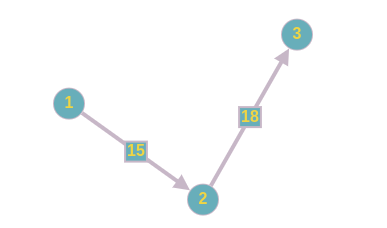
\includegraphics[scale=0.7]{img/example_3dim}
        \caption{3 sommets liés d'un graphe}
        \label{img_3somlinked}
    \end{figure}

    Ici, si $M$ est notre matrice d'adjacence, la valeur $M[1][2][3]$ sera égale au temps que mettra le robot à ramasser la balle 3, en sachant qu'il se situe actuellement sur la balle 2 et qu'il vient de ramasser la balle 1. Cette dernière information nous indique qu'il faut prendre en compte le fait que le robot doit effectuer une rotation de $90$° vers la gauche.

    \section{Deux approches différentes}
    \label{sec:diff_approch}
    a

    \subsection{Trouver la solution optimale}
    \label{subsec:sol_opti}

    Notre algoritme servant à calculer le chemin le plus court explore tout le chemins possibles et retourne le plus court. Pour cela, nous avons utilisé la fonction \verb|permutations()| du module \verb|itertools| afin d'obtenir un itérable de toutes les permutations de balles possibles. Chaque permutation correspond à un chemin possible. La complexité de cette fonction est en $O(n!)$, avec $n$ le nombre de balles.

    Ensuite, pour chaque permutation obtenue, nous allons calculer le poids total du chemin. Nous allons donc chercher $n$ fois le poids correspondant au déplacement voulu dans notre matrice d'adjacence. L'avantage de l'avoir définie telle qu'indiquée dans la partie \ref{sec:model_impl} se ressent ici puisque ces opérations se font en temps constant. Comme nous avons $n$ balles, et $n!$ permutations, trouver le chemin le plus court parmi toutes les permutations se fait en $O(n.n!) = O(n!)$.

    Au total, cet algorithme a une complexité factorielle, tout comme la résolution du problème du voyageur de commerce avec un approche naïve. Il faut donc s'attendre à ce que le temps de calcul augmente très vite au fur et à mesure que nous ajouterons des balles au problèmes.

    Pour réduire les opérations réalisées, lorsque nous suivons une permutation et que le poids, même si toutes les balles ne sont pas encore parcourues, dépasse le poids minimum des chemins précédemment parcourus, nous passons directement à la permutation suivante.

    \subsection{Approximer la solution}
    \label{subsec:sol_approch}
    a

    \section{Résultats}
    \label{sec:result}

    Nous avons fait tourner nos algorithmes sur de nombreux jeux de tests. Nous avons fait varier le nombre de balles afin de mesurer le temps pris par l'algorithme, ainsi que les vitesses de rotation et de déplacement du robot. Nous nous attendions à observer des comportements différents.

    \subsection{Solution optimale}
    \label{subsec:result_opt}

    Dans cette partie, nous étudierons les résultats obtenus avec l'algorithme de calcul du chemin optimal.

    La figure \ref{fig:timepathopt} montre le temps d'exécution (en échelle logarithmique) selon le nombre total de balles à ramasser. 

    \begin{figure}[H]
        \centering
        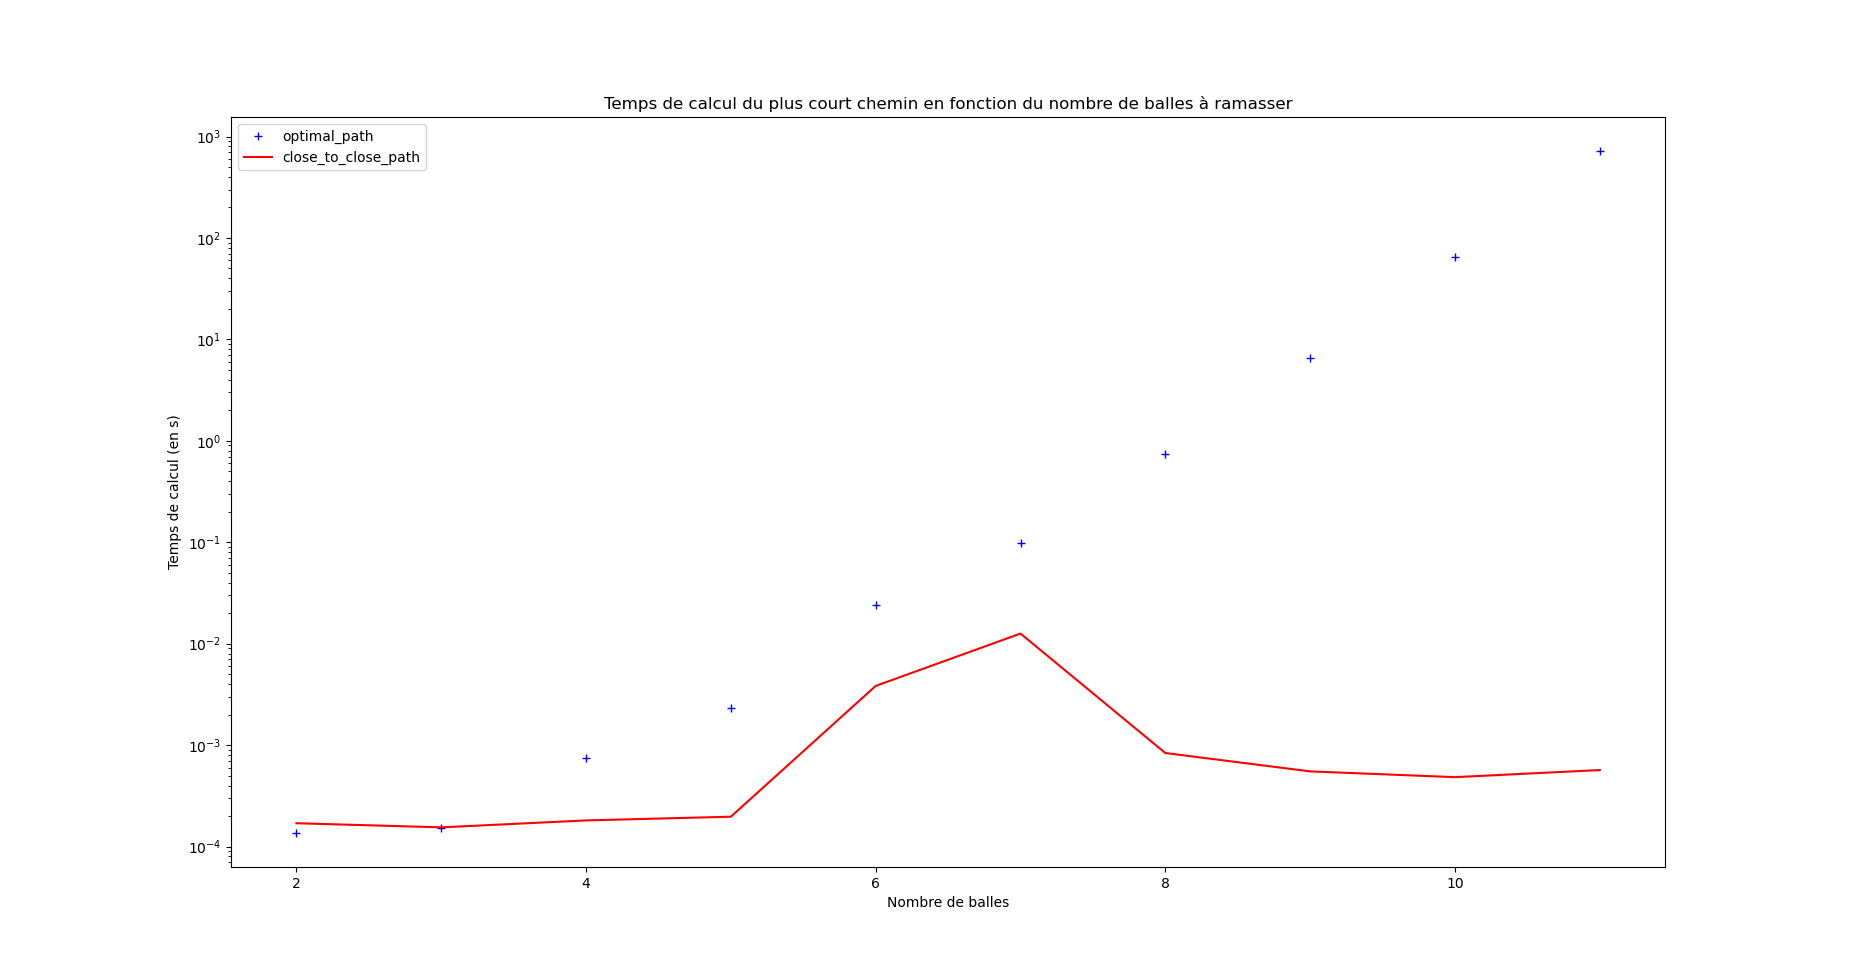
\includegraphics[width=\textwidth]{img/time_path_opt}
        \caption{Temps de calcul du plus court chemin en fonction de nombre de balles à ramasser}
        \label{fig:timepathopt}
    \end{figure}

    Nous remarquons bien que le temps de calcul augmente considérablement lorsqu'on rajoute une balle au monde. Il est de 14 secondes pour 10 balles, et de plus de 30 minutes pour 12 balles. Ceci nous montre bien les limites de ce genre d'algorithme, qui sont que, pour des problèmes de grande taille, le temps de calcul devient rapidement trop important. Cela est bien en adéquation avec notre étude de la complexité de cet algorithme.
    
    \medskip
    
    Ensuite, nous avons utilisé l'algorithme dans plusieurs mondes différents, en faisant varier les vitesses du robot. Lorsque la vitesse de déplacement était faible devant la vitesse de rotation, nous nous attendions à avoir un chemin minimisant la distance parcourue par le robot. A l'inverse, lorsque la vitesse de rotation était la plus faible, nous nous attendions à un chemin minimisant les angles lors du déplacement, c'est à dire un chemin le plus circulaire possible.

    Les figures \ref{subfig:terrain3mvt} (resp. \ref{subfig:terrain3rot}) donne le chemin le plus court obtenu lorsque la vitesse de déplacement (resp. de rotation) était plus grande que la vitesse de rotation (resp. de déplacement). L'étoile verte marque la position initiale du robot, tandis que le croix rouge représente la première balle ramassée.

    \begin{figure}[H]
        \centering
        \begin{subfigure}{0.35\textwidth}
          \centering
          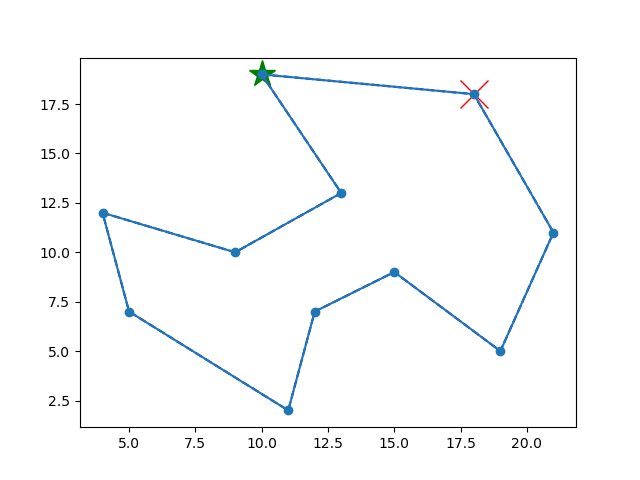
\includegraphics[width=\linewidth]{img/terrain3mvt}
          \caption{Vitesse de déplacement $<<<$ vitesse de rotation}
          \label{subfig:terrain3mvt}
        \end{subfigure}
        \hfill
        \begin{subfigure}{0.35\textwidth}
          \centering
          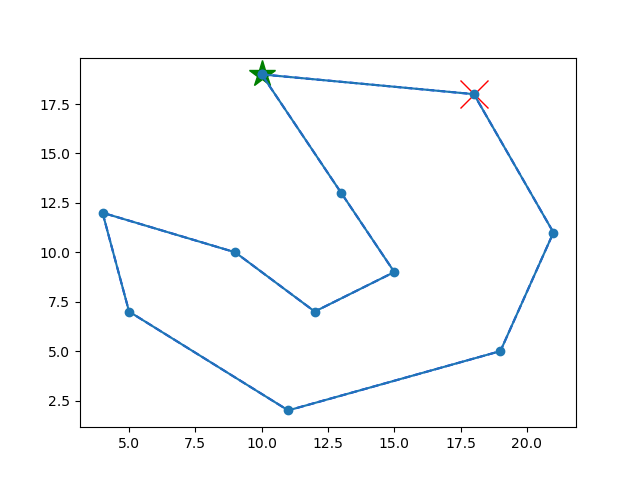
\includegraphics[width=\linewidth]{img/terrain3rot}
          \caption{Vitesse de rotation $<<<$ vitesse de déplacement}
          \label{subfig:terrain3rot}
        \end{subfigure}
        \caption{Chemins optimaux obtenus dans différentes situations}
        \label{fig:terrain3}
    \end{figure}

    Les chemins obtenus sont en adéquation avec les résultats attendus.

    \medskip

    Un exemple encore plus parlant est celui du monde fourni dans le sujet du projet. Dans les deux conditions énoncées précédemment, nous obtenons la figure \ref{fig:terrain2} :

    \begin{figure}[H]
        \centering
        \begin{subfigure}{0.35\textwidth}
          \centering
          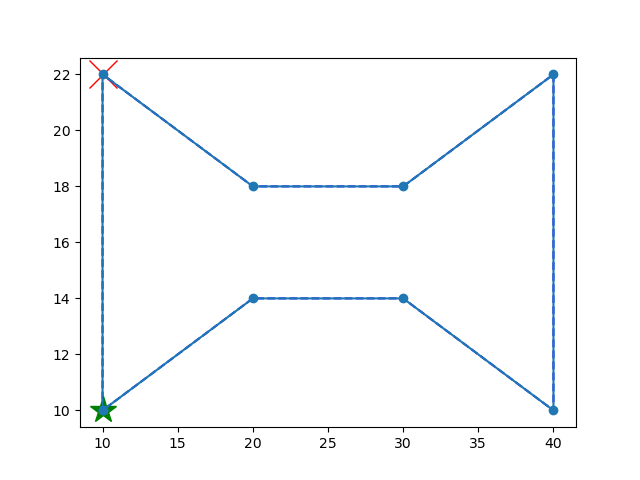
\includegraphics[width=\linewidth]{img/terrain2mvt}
          \caption{Vitesse de déplacement $<<<$ vitesse de rotation}
          \label{subfig:terrain2mvt}
        \end{subfigure}
        \hfill
        \begin{subfigure}{0.35\textwidth}
          \centering
          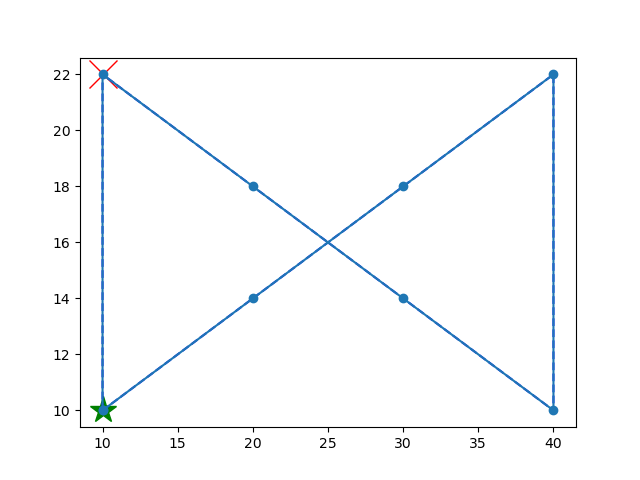
\includegraphics[width=\linewidth]{img/terrain2rot}
          \caption{Vitesse de rotation $<<<$ vitesse de déplacement}
          \label{subfig:terrain2rot}
        \end{subfigure}
        \caption{Chemins optimaux obtenus dans différentes situations}
        \label{fig:terrain2}
    \end{figure}

    Nous pouvons remarquer que les chemins reliant les 4 sommets de la partie gauche est identique dans les deuc situations (idem pour les 4 sommets de la partie droite). La seule différence se trouve au milieu.

    Il est facile de voir que la distance parcourue est plus petite dans la figure \ref{subfig:terrain2mvt}, tandis que les angles sont réduits au maximum dans la figure \ref{subfig:terrain2rot} (plus de lignes droites).

    \bigskip

    La taille du monde, elle, n'a aucun impact sur les résultats. En effet, les sommets de notre graphe sont uniquement les balles à ramasser, donc la taille totale du monde n'a aucune incidence (sauf s'il devient trop petit et donc que certaines balles ne soient pas à considérer).

    \subsection{Solution approchée}
    \label{subsec:result_approch}

    \section{Conclusion}
    \label{sec:ccl}

\end{document}